\section{Methods} \label{sec:methods}

After opening with a brief primer on hereditary stratigraphy and an overview of application in proposed ``gene-'' and ``species-level'' instrumentation (Section \ref{sec:genome-instrumentation}), discussion in this section turns to cover debuted inferential techniques and corresponding validation experiments.
Three inferential techniques are described:
\begin{enumerate}
\item genealogical inference (Section \ref{sec:genealogical-inference}),
\item effective population size inference (Section \ref{sec:population-size-inference}), and
\item positive selection inference (Section \ref{sec:selection-inference}).
\end{enumerate}

The first two rely on ``species-level'' annotation.
The third, selection inference, applies ``gene-level'' instrumentation.
Section \ref{sec:software-data} closes with information on software implementation and supplementary materials.

\subsection{Genome Instrumentation}
\label{sec:genome-instrumentation}

This section reviews hereditary stratigraphy as originally developed for inference over asexual populations then introduces gene- and species-level hereditary stratigraphy instrumentation strategies designed for sexual populations.
Subsequent discussion covers recombination and ``gene drive'' mechanisms employed for species-level instrumentation.


% \begin{figure}
  \centering
  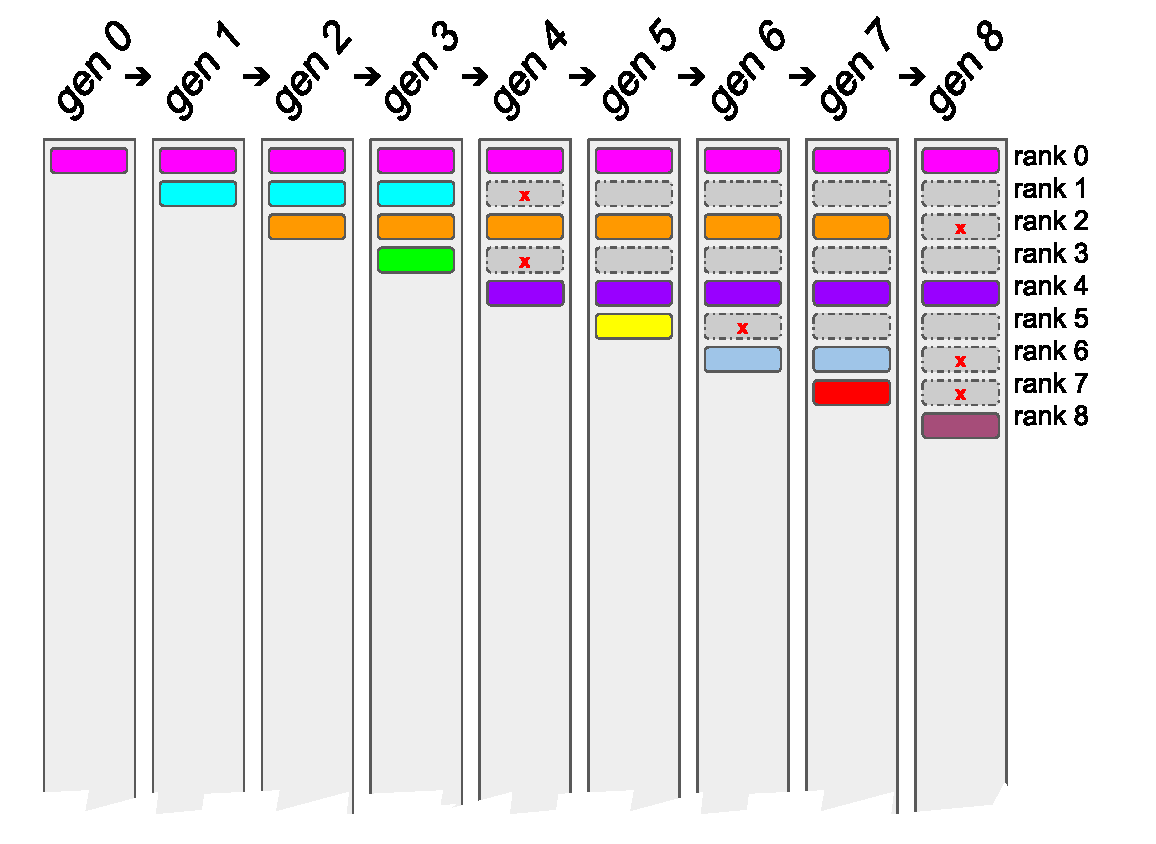
\includegraphics[width=\textwidth]{img/deposit-prune-example}
  \caption{
    TODO
  }
  \label{fig:deposit-prune-example}
\end{figure}

% \begin{figure}
  \centering
  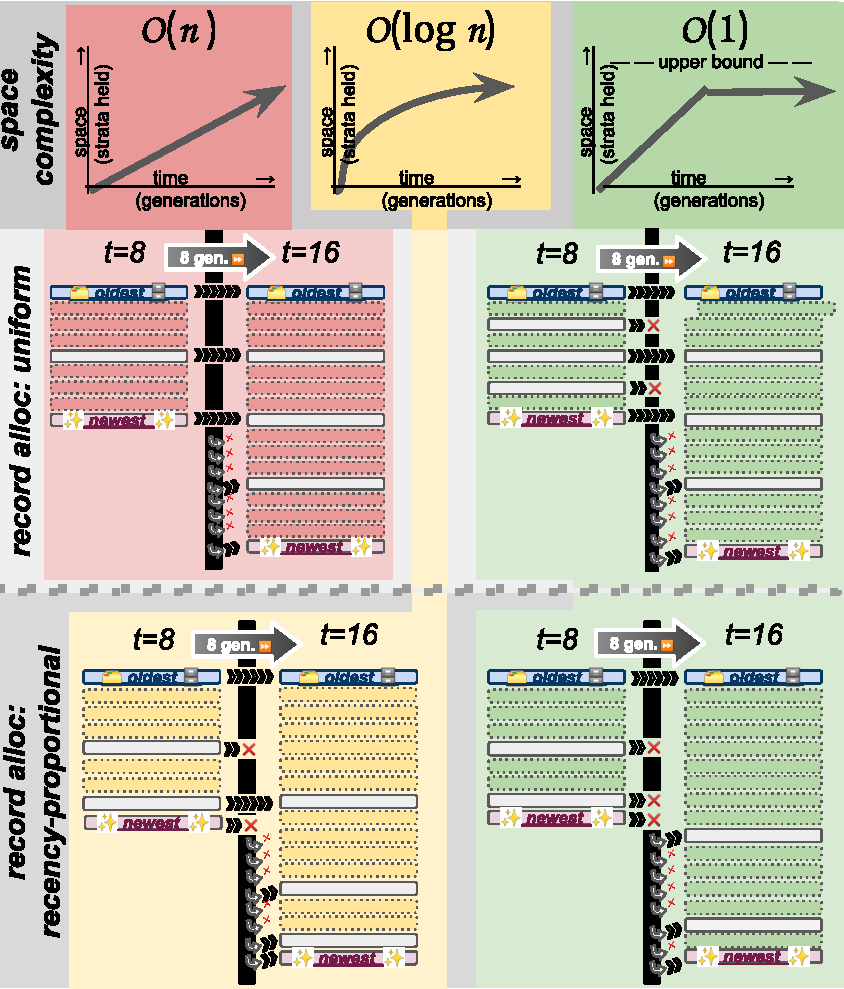
\includegraphics[width=\textwidth]{img/retention-policy-matrix}
  \caption{
    Comparison of four stratum retention policies by space complexity per stratigraph with respect to generations elapsed (columns, red/yellow/green) and by distribution of retained differentia (rows).
    Uniform allocation keeps differentia in evenly-spaced layers.
    Recency-proportional allocation keeps more more-recent differentia, trading off coarser resolution to infer ancient phylogenetic events for finer resolution to infer recent phylogenetic events.
    Retained layers under each policy are shown at $t=8$ generations and $t=16$ generations, with new differentia being deposited in a descending fashion.
    Differentia pruning events are noted with a red $x$.
  }
  \label{fig:retention-policy-matrix}
\end{figure}

\textbf{Hereditary Stratigraphy.}
Proposed methods for genealogical and evolutionary inference over distributed sexual populations draw on ``hereditary stratigraphy,'' originally developed to facilitate phylogenetic inference over asexual populations \citep{moreno2022hstrat}.
The core mechanism of this technique is generation-on-generation accumulation of randomized ``fingerprint'' packets.
Offspring inherit parents' fingerprints and append a new entry.
This process repeats with the next generation.

Each accumulated fingerprint ultimately serves as a kind of linealogical checkpoint.
Because fingerprints are faithfully inherited each generation after their creation, discrepancy between coincident fingerprints held by two population members implies divergent ancestry at their shared time point.
So, last common ancestry necessarily precedes the first mismatching fingerprints.
Fingerprint values convey no function phenotypic information.
Rather, they should be considered simply as neutral ornamentation affixed to an underlying functional genome to instrument it.
Because they tag along with genomes across replication events, a system's phylogenetic history can be reconstructed by proxy based on these instruments.

Some attention must be paid to memory footprint.
Proceeding naively, fingerprint accumulation with each generation would hopelessly bloat annotation size.
Fortunately, the underlying inferential mechanism supports thinning out of fingerprints.
Pruned-away fingerprints introduce uncertainty into estimation of two records' divergence generation.
If every other fingerprint was pruned, for example, divergence generations would only be estimable to within 2 generations.
In this way, configuration of what fingerprints to keep when directly administers underlying trade-offs between memory use and inferential power.
Although beyond present scope, significantly more can be said about fingerprint curation.
For detail, refer to \citep{moreno2022hereditary}.

To simplify experimental setup and analysis, experiments reported here do not incorporate fingerprint pruning.
However, all inference mechanisms introduced here are, in principle, compatible with fingerprint pruning.
Further work remains to directly investigate how pruning affects presented approaches' characterization of evolutionary history and dynamics.
Analogous work in asexual populations should provide some initial indications in this direction \citep{moreno2023toward}.

This work uses 64 bit fingerprints, which collide spuriously with negligible probability $2^{-64} \approx 5 \times 10^{-20}$.
At population size 100 over 200 generations, as in the first sets of reported experiments, the probability of any collision is miniscule: $< 2 \times 10^{-15}$.
At population size 200 over 400 generations, as in the last set of reported experiments, the probability of any collision is also miniscule: $< 5 \times 10^{-15}$.

\begin{SCfigure}[3][b]
  \centering
  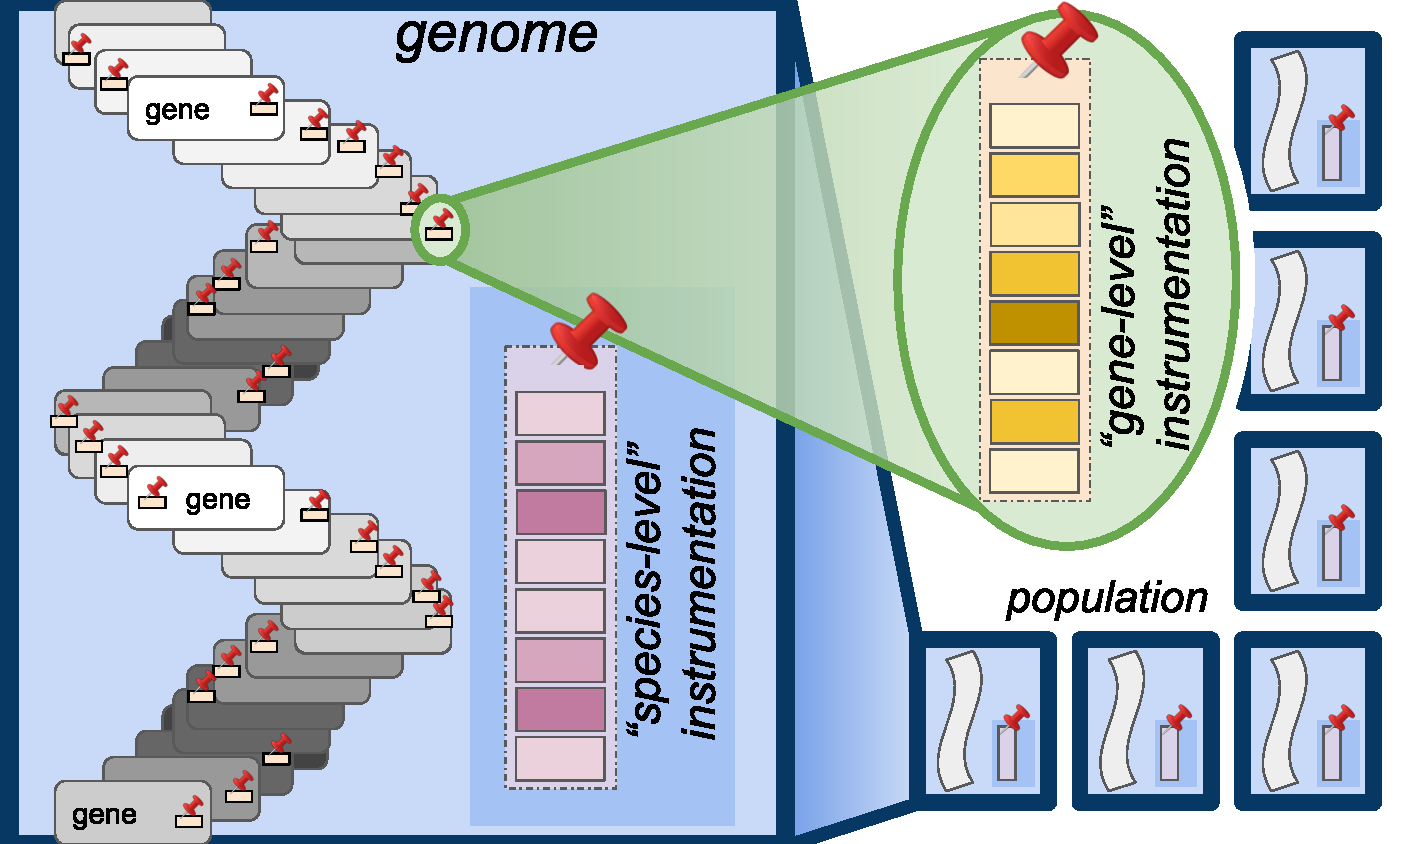
\includegraphics[width=0.5\textwidth]{img/annotation-types}
  \caption{
    Proposed instrumentation methods: ``species-level'' and ``gene-level'' instrumentation.
    Each organism has a single hereditary stratigraph attached as species-level instrumentation, with a gene drive mechanism (Figure \ref{fig:gene-drive}) ensuring consistentcy within species (i.e., interbreeding populations).
    Gene-level instrumentation associates instrumentation with individual genes, to be used for gene tree reconstructions.
  }
  \label{fig:annotation-types}
\end{SCfigure}

\textbf{Sexual Instrumentation Schemes.}
As originally devised for asexual populations, hereditary stratigraph annotations assign one-to-one with genomes.
Here, we explore two alternate schemes designed for instrumentation of sexual populations: ``gene-level'' and ``species-level'' instrumentation.
Figure \ref{fig:annotation-types} compares these two schemes.

Gene-level instrumentation views individual genes simply as asexual atoms, and instruments them individually.
Reconstructions, therefore, operate along the lines of ``gene tree'' analsyes in traditional phylogenetics \citep{avise1989gene}.
In some cases, it may make sense to instrument every gene independently.
Other applications may warrant instrumenting only a subset of genes or introducing instrumented ``dummy'' genes.

Species-level instrumentation associates one instrument per genome but these instruments adopt a consensus value within species populations.
Consensus arises through a ``gene drive'' mechanism (described below) that forces a single fingerprint value to sweep each fingerprint layer within an interbreeding subpopulations.

Species-level instrumentation powers genealogical inference (Section \ref{sec:genealogical-inference}) and population size inference (Section \ref{sec:population-size-inference}).
Gene hereditary stratigraph instrumentation powers positive selection inference (Section \ref{sec:selection-inference}).

\begin{SCfigure}[3][b]
  \centering
  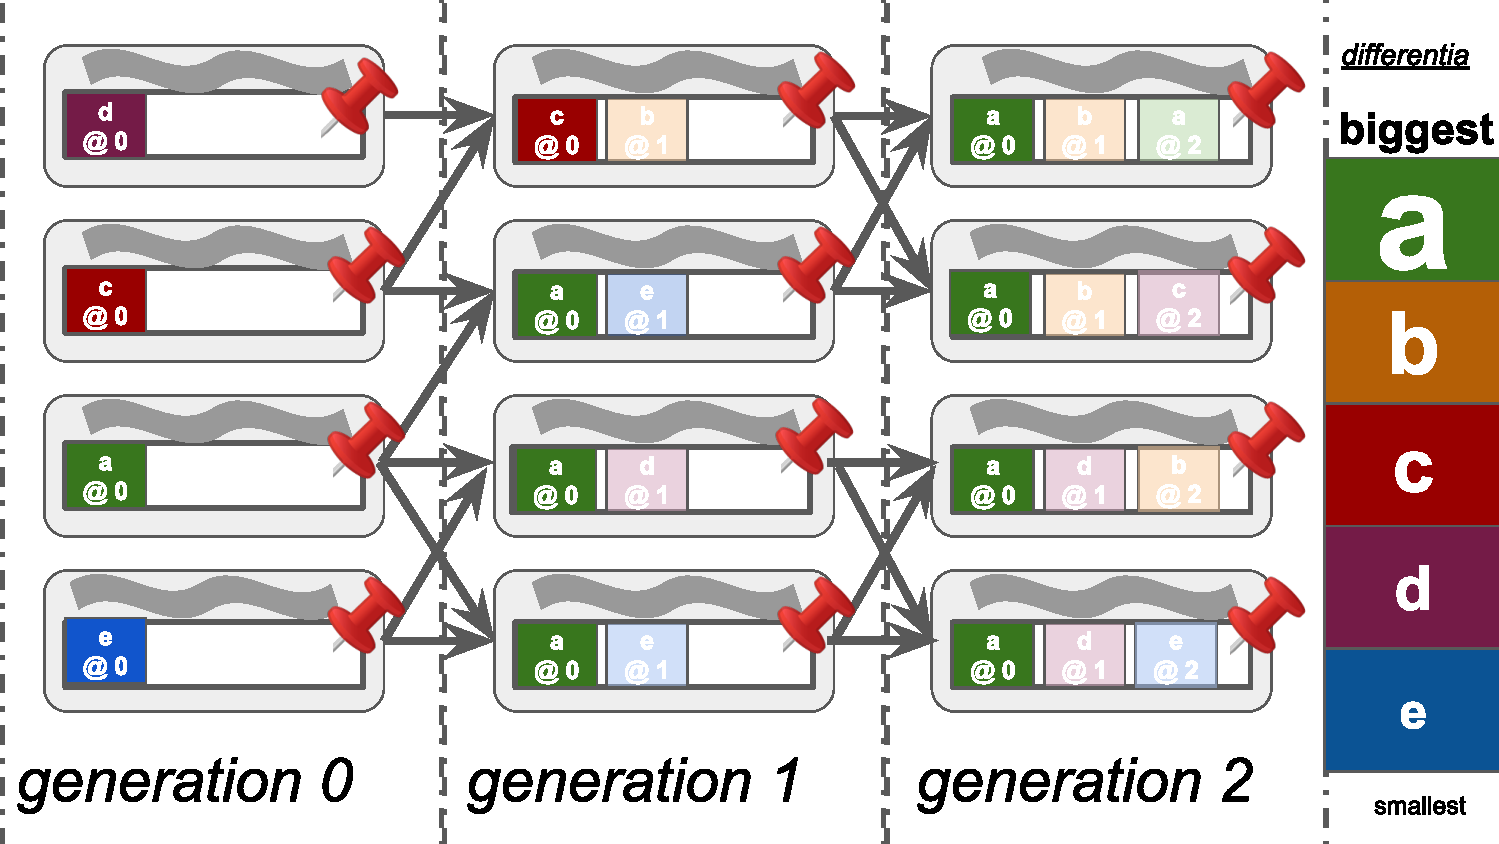
\includegraphics[width=0.6\textwidth]{img/gene-drive}
  \caption{
    Gene drive mechanism for species-level instrumentation.
    The larger of parents' differentia values at each layer is inherited.
    The largest value generated among layer 0 differentia ($a$) spreads from one member at generation 0 to all four by generation 2.
    This mechanism applies to ``species-level'' instrumentation (Figure \ref{fig:annotation-types}).
  }
  \label{fig:gene-drive}
\end{SCfigure}

\textbf{``Gene-drive'' Recombination Mechanism.}
Species-level tracking relies on consensus among fingerprint values within reproductively isolated subpopulations.
Drift will ultimately yield consensus, but expected coalescence times can be long for large populations
A simple inheritance rule reaches consensus faster: inherit the larger of parents' fingerpint values.
Global maximum fingerprint values will spread rapidly and fix.
Figure \ref{fig:gene-drive} depicts this mechanism.

Asynchronous generations slightly complicate the picture.
When individuals from different generations recombine, one parent will have fingerprint layers absent in the other.
How should recombination proceed in this case?
One possibility would be to simply ``fast forward'' the younger instrument to match the generational depth of the elder.
However, like with fingerprint pruning above, full consideration remains for future work.
All reported experiments use synchronous generations.

The gene-drive-based recombination mechanism described in this section applied exclusively to species-level instrumentation.
(Gene-level instruments, although tagging along with genes shuffled up through genome-level recombination, did not themselves recombine.)

\textbf{Fingerprint Collision Probability.}
Under gene-drive recombination, fixed fingerprints skew large due to the gene drive criterion.
This skew increases the probability of fingerprint collision between two populations which would cause spurious detection of shared ancestry.
We will assess the extent of this issue by computing threshold population sizes where collision probability becomes substantive.

Suppose independent populations of size $a$ and $b$.
The largest fingerprint in each population will drive to fixation.
If each population members' gene is drawn from uniform distribution on integers $[0, u)$, then the probability of collision between the populations' fixed genes can be derived as

\begin{scriptsize}
\begin{align*}
\frac{a}{a + b}\sum_{n=1}^{a + b - 1} \frac{u^{- n - 1} \left(\frac{u - 1}{u}\right)^{a + b - n - 1} \left(1 - \frac{{\binom{a - 1}{n}}}{{\binom{a + b - 1}{n}}} \right) {\binom{a + b}{n + 1}}}{1 - \left(\frac{u - 1}{u}\right)^{a + b - 1}}
+ \frac{b}{a + b} \sum_{n=1}^{a + b - 1} \frac{u^{- n - 1} \left(\frac{u - 1}{u}\right)^{a + b - n - 1} \left(1 - \frac{{\binom{b - 1}{n}}}{{\binom{a + b - 1}{n}}} \right) {\binom{a + b}{n + 1}}}{1 - \left(\frac{u - 1}{u}\right)^{a + b - 1}}.
\end{align*}
\end{scriptsize}
% Derivation will be provided in supplementary materials. TODO?

For 32-bit differentia $u = 2^{32}$, collision occurs with $p < 0.5$ ($p = 0.46$) for populations of size $a = b = 2^{32}$.
Collision occurs with $p < 0.01$ for populations of size $a = b = 2^{26}$.
So, 32-bit fingerprints can differentiate species pairs of around $6.7 \times 10^{7}$ members each with reasonable consistency.%
\footnote{
Reported experiments used 64-bit fingerprint values, which will exhibit even lower collision probabilities.
However, numerical considerations impede precise calculation.
}


\subsection{Genealogical Inference}
\label{sec:genealogical-inference}

Sections \ref{sec:allopatry-treatment,sec:ring-treatment,sec:bag-treatment} describe the three treatments compared to test the proposed genealogical inference mechanisms.
Section \ref{sec:phylogeny-extraction} lays details the procedure used to convert recorded sexual pedigrees to phylogenetic trees that reconstruction quality could be evaluated against.

This experiment tested the quality of genealogical history recovered from species-level hereditary stratigraph annotation.
Phylogenetic reconstruction quality was tested over three evolutionary treatments.
The first, ``allopatry,'' covered full speciation through introduction of a strict reproductive barrier among subpopulations.
The second, ``ring,'' covered partial phylogenetic structure over subpopulations linked through small amounts of migration.
A third --- as a control --- was designed to lack meaningful phylogenetic structure at all due to well-mixed interbreeding ensuring close relatedness between all population members.
Ten independent replicates were performed for each treatment.

The experiment was performed on the one-max problem domain described in Section \ref{sec:one-max}.
After the 200th and final generation, the species-level annotations extracted from each of the extant organisms.
Phylogenetic structure was reconstructed using from these annotations using the agglomerative trie-based reconstruction techniques developed in \citep{moreno2023toward}.
(Essentially, the phylogeny is constructed so that organisms track the lineage they share the most consecutive ``fingerprint'' differentia with and then branch out at the point of the first disparity in differentia value.

To evaluate reconstruction quality, inferred phylogenies were compared to references extracted directly from underlying sexual pedigree record of the simulation using the MRCA-based UPGMA methods described in Section \ref{sec:phylogeny-extraction}.
Disagreement between reconstruction and reference was quantified using the quartet tree distance metric \citep{estabrook1985comparison}.

Additionally, inferred phylogenies were visualized to confirm whether reconstructions recovered the major features of treatments' evolutionary histories.

\subsubsection{Allopatry Treatment}
\label{sec:allopatry-treatment}

This treatment simulates 100 generations of well-mixed sympatric evolution.
At generation 100, the population is divided into two 50-member subpopulations.
These subpopulations evolve independently with no migration for 50 generations.
Then, at generation 150, the first subpopulation is split again into five 10-member subpopulations.
The remaining 50-member subpopulation and the five new 10-member subpopulations then evolve independently with no migration for a further 50 generations.
Phylogenetic reconstruction from this treatment should ideally recover a binary branching at generation 100 followed by a secondary quintuple-branching along one lineage at generation 150.

\subsubsection{Ring Treatment}
\label{sec:ring-treatment}

This treatment splits the population into ten distinct subpopulations (islands), each of which evolved independently.
The subpopulations were arranged in a ring topology, and one individual migrated between adjacent populations per generation happens once per generation.

\subsubsection{Bag Treatment}
\label{sec:bag-treatment}

This treatment selects and recombines individuals uniformly from across the entire population.
As such, all individuals extant at simulation completion are closely related so no meaningful phylogenetic structure exists to be detected.

\subsubsection{Phylogeny Extraction from Pedigree Records}
\label{sec:phylogeny-extraction}

In order to provide a baseline reference to evaluate annotation-based phylogenetic reconstructions against, phylogenetic relationships between extant organisms (i.e., an asexual tree describing ``relatedness'') were extracted from sexual pedigrees (i.e., a reticulated directed acyclic graph describing ancestry).

Such conversion has fundamental limitations: in well-mixed populations of modest size, structured differences in phylogenetic relatedness do not meaningfully exist.
However, speciation and spatial structure can introduce meaningful aspects of phylogenetic structure.

A naive technique was used to distill phylogenetic relationships from pedigree data.
Most Recent Common Ancestors (MRCA) were computed pairwise from the pedigree data to construct a distance matrix among extant individuals.
Unweighted Pair Group Method with Arithmetic mean (UPGMA) reconstruction based on this distance matrix yielded inferred phylogenetic structure \citep{sokal1958university}.
Finally, corrections to branch lengths were performed to accurately position the terminal nodes (i.e., extant organisms) at their known generational depths.

No effort was made to cluster extant organisms into taxa based on a relatedness threshold, so reconstructions contained non-informative branch structure among closely-related individuals.


\subsection{Population Size Inference}
\label{sec:population-size-inference}

This section introduces the mechanistic principle behind distributed population size estimation, reports statistical formulations derived to this end, then describes experiments that test the proposed inference technique.

\textbf{Inference Principle.}
Recall that the proposed gene drive mechanism (Section \ref{sec:genome-instrumentation}) fixes the maximum of population size $n$ fingerprint values, each drawn from a uniform distribution.
Under this gene drive mechanism, fixed fingerprint magnitude reveals information about population size: larger populations tend to fix greater fingerprints (as illustrated in Supplementary Figure \ref{fig:beta-explain}).
Scaling integer fingerprint values to fall between 0 and 1, fixed fingerprint magnitude turns out to follow beta distribution $\beta(n, 1)$ \citep{gentle2009computational}.

Directly analogous techniques to estimate population size have also arisen in decentralized, anonymous network engineering \citep{varagnolo2010distributed,hakan2012distributed}.
In these schemes, nodes independently draw a random vector of numerical values from a known distribution.
Values are exchanged through an aggregating function (e.g., minimum, maximum, etc.), ultimately resulting in consensus values fixed within the network.
Each node can then independently infer probabilistic information about the larger network, in a manner that is generally consistent across nodes.

\textbf{Population Size Estimator Statistics.}
Statistical details for population size inference follow, some of which are, to best knowledge, not yet reported.
Natural log is used throughout.
Section \ref{sec:software-data} links to full derivations.

\textit{Maximum Likelihood Estimator (MLE).}
The maximum likelihood estimator for population size given $k$ independent observations of unit-scaled fixed-fingerprint values $x_i$ is
\begin{footnotesize}
\begin{align} \label{eqn:popsize_mle}
\hat{n}_\mathrm{mle} = -k/\textstyle\sum_{i=1}^k \log( x_i ).
\end{align}
\end{footnotesize}

With true population size $n$, mean square error of the estimator is $\mathrm{MSE}(\hat{n}_\mathrm{mle}) = n^2 (k^{2}+ k-2) / [(k-1)^{2}(k-2)]$.
Expected value follows as $\mathrm{E}(\hat{n}_\mathrm{mle}) = nk/(k-1)$ for $k>1$.
Subtracting this value from $\hat{n}_\mathrm{mle}$ yields a mean-unbiased population size estimator.
These MLE results were also derived in \citep{varagnolo2010distributed}.

\textit{Confidence Interval.}
Confidence intervals are useful to interpretation of population size estimates.
Formulations derived from the maximum likelihood estimator are provided below.

For a single observation of unit-scaled fixed-fingerprint magnitudes $\hat{x}$, the population size $n$ can be estimated with $c\%$ confidence to fall between lower bound $\log[(50+0.5c)/100] / \log\hat{x}$ and upper bound $\log[(50-0.5c)/100] / \log\hat{x}$.
At this low observational power, the 95\% confidence interval spans a 145-fold order of magnitude and a 99\% confidence interval spans a 1057-fold order of magnitude.

For $k$ observations of unit-scaled fixed-fingerprint magnitudes $\hat{x}_i$, population size can be estimated with $c\%$ confidence to fall within the interval $(\hat{n}_\mathrm{lb}, \, \hat{n}_\mathrm{ub})$, computed as numerical solutions of

\begin{footnotesize}
\begin{align}
0
= 2\Gamma\Big(k, -\hat{n}_\mathrm{lb}\sum_{i=1}^k \log\hat{x}_i\Big) - \Gamma(k)\frac{100+c}{100} \text{ and }
0
= 2\Gamma\Big(k, -\hat{n}_\mathrm{ub}\sum_{i=1}^k \log\hat{x}_i\Big) - \Gamma(k)\frac{100-c}{100}.  \label{eqn:popsize_mle_ci}
\end{align}
\end{footnotesize}

Here, $\Gamma$ is the complete gamma function.
Four independent observations provide a 95\% confidence interval spanning 8-fold magnitude or a 99\% confidence interval spanning a 16-fold magnitude.
Nine independent observations are sufficient for a 95\% confidence interval spanning a factor spanning 4-fold magnitude or a 99\% confidence interval spanning a factor of 6-fold magnitude.
Thirty-three independent observations are sufficient for a 95\% confidence interval spanning 2-fold magnitude or a 99\% confidence interval spanning 2.5-fold magnitude.
Because $\sum_{i=1}^k \log\hat{x}_i \propto \hat{n}_\mathrm{mle}^{-1}$, confidence bound width can be shown to scale as a constant factor of population size $n$.

\textit{Median-unbiased Estimator.}
Evaluating either confidence interval formula with $c = 50$ derives a median-unbiased estimator.

\textit{Credible Intervals.}
Assuming a uniform prior over population size, credibility contained within a factor $f$ of the maximum likelihood estimate $\hat{n}_\mathrm{mle}$ can be calculated as $\gamma(k + 1, f k)/k! - \gamma(k + 1, k/f)/k!$.
Here, $\gamma$ is the lower incomplete gamma function.
By form, this credibility remains constant across population sizes $n$.
Credibility interval width scales similarly with sample size as discussed above for confidence intervals.

\textit{Rolling Estimation.}
Experiments reported here compute a population size estimate and confidence intervals from a simple rolling collection of ten preceding fixed-gene magnitudes.
Supplemental Section \ref{sec:population-size-inference-example} walks through an example of rolling population size inference.
More sophisticated regularizations have been proposed to estimate dynamically-changing population sizes from time series data \citep{hakan2012distributed}.

\textbf{Validation Experiment.}
This experiment tests ability of the population size estimation process to detect differences between populations and to detect changes within a population over time.
Four treatments were evaluated with ten independent replicates performed per treatment.

\textit{Bottleneck treatment.}
Simulated population crash and rebound.
Population size was kept at 100 for 67 generations, reduced an order of magnitude to 10 for 66 generations, and then returned to 100 for another 67 generations.

\textit{Range expansion.}
Simulated gradual population size growth.
Population size was initiated at at 10 for 67 generations, then increased linearly for 66 generations to 142 at generation 133, and then maintained at 142 for another 67 generations.

\textit{Selection-pressure.}
Modulated selection intensity.
This affects effective population size by changing the number of population members eliminated without contributing to the gene pool.
High selection pressure was applied for 67 generations (tournament size 8). Then, selection pressure was eliminated for 66 generations (tournament size 1).
Finally, high selection pressure was reinstated for the last 67 generations (tournament size 8).

\textit{Control treatment.} Constant population size 100 for 200 generations.


\subsection{Positive Selection Inference}
\label{sec:selection-inference}

This section presents proposed gene selection inference methods and design of validation experiments used to test it.

\begin{sidewaysfigure}
  \centering
  \begin{minipage}{.7\textwidth} % adjust the width as needed

    \begin{minipage}{\textwidth}
      \centering
      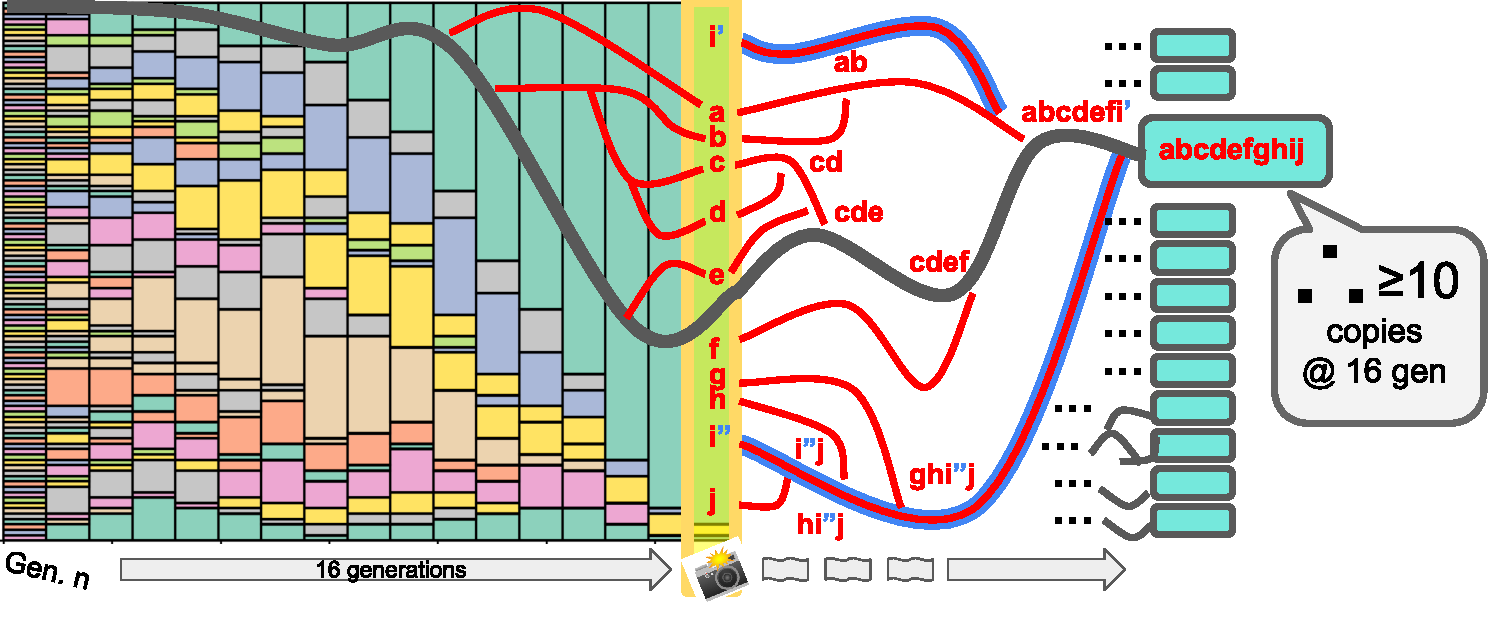
\includegraphics[height=0.30\textheight]{img/copy-count-snapshot}
      \subcaption{Cartoon depiction of delayed copy count estimation mechanism, annotated over Muller plot depicting weak selection over focal allele.
      }
      % \label{fig:ne-example-replicates:bottleneck}
    \end{minipage}%

    \vspace{1cm}

    \begin{minipage}{0.5\textwidth}
      \centering
      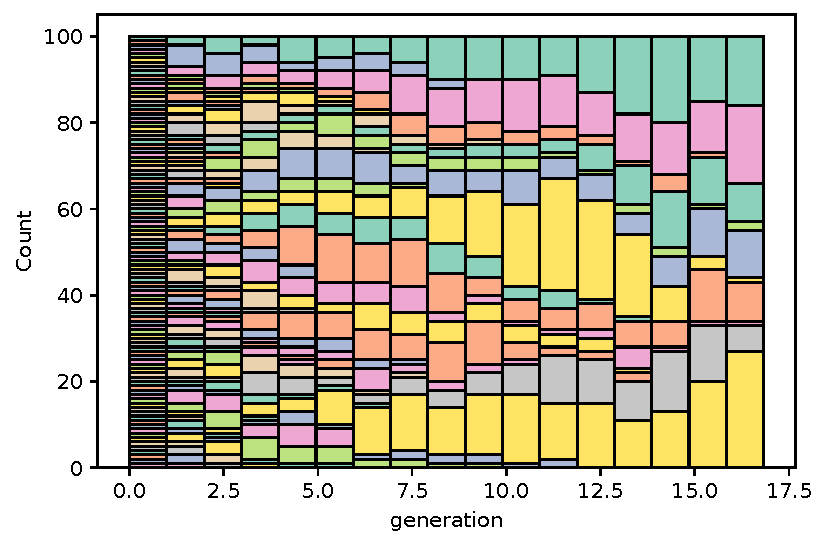
\includegraphics[height=0.2\textheight]{notebooks/notebooks/teeplots/fit=0.0+hue=clade+multiple=stack+ngen=16+npop=100+palette=set2+viz=histplot+x=generation+ext=}
      \subcaption{Muller plot depicting no selection for focal allele, ending with smaller copy count after 16 generations.}
      % \label{fig:ne-example-replicates:selection_pressure}
    \end{minipage}%
    \begin{minipage}{0.5\textwidth}
      \centering
      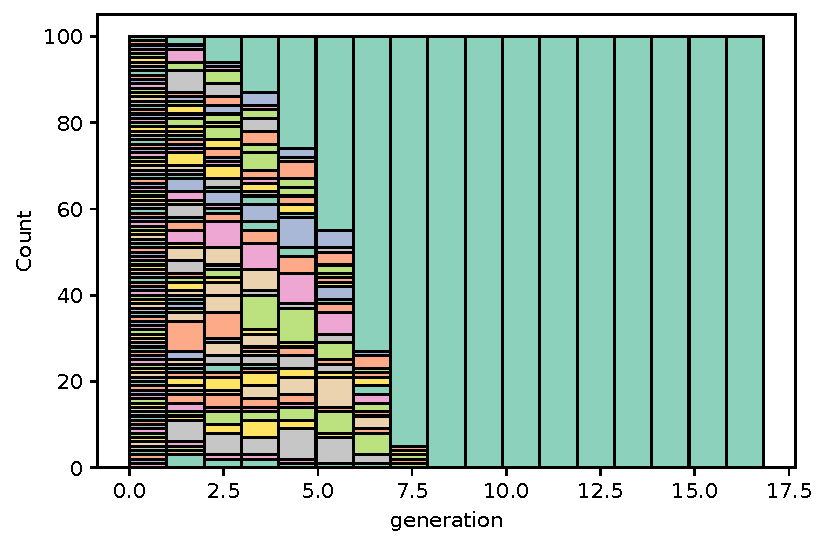
\includegraphics[height=0.2\textheight]{notebooks/notebooks/teeplots/fit=1.0+hue=clade+multiple=stack+ngen=16+npop=100+palette=set2+viz=histplot+x=generation+ext=}
      \subcaption{Muller plot depicting strong selection for focal allele, with fixation occuring before 16 generations.}
      % \label{fig:ne-example-replicates:control}
    \end{minipage}

  \end{minipage}
  \hfill % Creates horizontal space. Can also use \hspace{<len>}
  \begin{minipage}{.25\textwidth} % adjust the width as needed
    \caption{
      Proposed mechanism for detecting gene-level selection via a distributed delayed copy count estimation mechanism.
      Strata deposited at generation $n$ progress through 16 generations, with copy count of one allele growing due to selection.
      On the sixteenth generation, a ``snapshot'' is performed to set a random bit on field annotated onto each descendant differentia copy.
      In subsequent recombination events, set bits are exchanged between bit fields associated with common differentia.
      Copy count at generation $n + 16$ from can then estimated from these bit fields, with high copy count being suggestive of selection.
      Note that in this example collision between set bits $i'$ and $i"$ result in an undercount.
      This mechanism is associated with ``gene-level'' instrumentation (Figure \ref{fig:annotation-types}).
    }
    \label{fig:ne-example-replicates}
  \end{minipage}

\end{sidewaysfigure}


% notebooks/notebooks/teeplots/notebook=ne-inference+replicate=0+treatment=bottleneck+viz=plot-running-estimation+x=rank+y=population-size+ext=.pdf
%
% notebooks/notebooks/teeplots/notebook=ne-inference+replicate=0+treatment=control+viz=plot-running-estimation+x=rank+y=population-size+ext=.pdf
%
% notebooks/notebooks/teeplots/notebook=ne-inference+replicate=0+treatment=range-expansion+viz=plot-running-estimation+x=rank+y=population-size+ext=.pdf
%
% notebooks/notebooks/teeplots/notebook=ne-inference+replicate=0+treatment=selection-pressure+viz=plot-running-estimation+x=rank+y=population-size+ext=.pdf

\textbf{Inference Mechanism.}
Alleles experiencing positive selection increase in frequency.
However, allele frequency increases can also occur through drift.
The key difference between the two is the \textit{rate} of increase --- drift tends to be slower than selection, especially for large population sizes.

Selection can therefore be differentiated from drift dynamics by considering copy count of gene descendants after a fixed number of generations $g$.
If this copy count exceeds expectation under a null hypothesis of pure drift dynamics, positive selection can be inferred.
Stronger positive selection will correlate with greater growth of copy count within the $g$ generation window.
This is the working principle behind the proposed detection method.

The proposed mechanism measures delayed copy count through gene-level instrumentation.
Each fingerprint is bundled with a fixed-length, zero-initialized bit field.
These bit fields are copied verbatim to descendants along with the rest of gene annotations.

At the $g$th generation following its creation, a single bit is set at random in each bit field.
During subsequent recombination, corresponding bit fields with matching fingerprints combine using the bitwise or operation.
In this manner, set bits propagate among the records that trace back to a particular founder gene at the snapshot window outset.
Annotations' bit counts converge to reflect the number of gene copies present after generational delay $g$.
Figure \ref{fig:copy-count-snapshot} summarizes the overall mechanism.
Set bits can undercount snapshot gene copies due to bit position overlap or gene copy extinctions subsequent to generation $g$.
Sensitivity to larger copy counts could be achieved by setting bits instead with probability $p < 1$.

A bit field width of 8 bytes and a snapshot delay of 16 generations, by arbitrary choice, were used in experiments.
Better sensitivity to weak selection events should be achievable through longer snapshot windows and larger bit fields, but potentially at the cost of diluting signal from strong selection events.
Future work should explore how to best tailor snapshot window length and bit field widths.

Soft sweeps should, in principle, be detectable to some extent through this methodology, as they involve increases in copy count at faster-than-drift rates.
Soft sweeps are scenarios where changes in environmental conditions induce positive selection on an existing, potentially widespread allelic variant that was previously neutral \citep{hermisson2005soft}.
However, weak sweeps on very-widespread alleles will register only a weak signal on this instrumentation because increases in copy count are spread across many preexisting allele copies.
Although weak sweeps are not explored here, they merit future consideration.

\textbf{Validation Experiment.}
A minimalistic experimental system was devised.
Each individual in the population comprised a single floating-point number, representing a single focal gene.
Gene values were restricted between 0.0 and 1.0.
Fitness score was defined as the sum of the genetic value and a random number drawn from a continuous, uniform unit-valued distribution.
So, individuals' gene value corresponded directly to probabilistic fitness advantage.
For example, a value of 0.2 would give an average 20\% selective advantage.
Fitness scores for each individual were calculated once per generation and used for all tournaments.

All individuals were initialized with gene value 0.0.
At generation 50, one organism's gene value was set to either 0.0,\footnote{The smallest representable floating point value was set for fitness advantage treatment 0.0 so the introduced gene could be differentiated from the background gene.
This value was small enough as to have no meaningfully detectable effect on selection.} 0.1, or 1.0.
This operation was repeated at subsequent generations if the introduced allele went extinct.
This procedure enabled comparison of a strong selective sweep (fitness advantage 1.0), a weaker selective sweep (fitness advantage 0.1) and a control treatment with pure drift dynamics (fitness advantage 0.0).

Synchronous selection with tournament size 2 was performed over 200 simulated generations with constant population size of 400.
Crossover propagated a random parent's gene value.
No mutation was applied.
Ten independent replicates were performed of each treatment.


\subsection{Software \& Data}
\label{sec:software-data}

Software, data, analyses, and supplementary materials are hosted via the Open Science Framework at \url{https://osf.io/xj5pn/}.

Data structures and algorithms associated with hereditary stratigraphy methodology are published in the \texttt{hstrat} Python package on PyPi and at \url{github.com/mmore500/hstrat} \citep{moreno2022hstrat}.
Recombination features and corresponding C++ implementations are on the project's roadmap.

This work benefited greatly from open source scientific software \citep{cock2009biopython,fortin2012deap,sand2014tqdist}.
The Alife data standard facilitated tool interoperation \citep{lalejini2019data}.
